% !TeX root = ../main.tex
% Add the above to each chapter to make compiling the PDF easier in some editors.

\chapter{Related Work}\label{chapter:literature}
The building pillars of this thesis is the research around Kubernetes, IoT and Unikernels. Kubernetes has a very active community around it, both in research and development, that Google Scholar returns 9.140 results when searching the technology. While Kubernetes has many resources, a Google scholar search on Unikernels brings 1150 results. Most of those results focus on benchmarking unikernels with other virtualisation methods. There are some unikernel-orchestration projects as well. Following sections include some projects regarding those topics.

\section*{Kubernetes}

There is an ongoing research on migrating Kubernetes to different domains other than container management such as managing virtual machines using Kubernetes instead of tools like Puppet, Chef or Ansible. The KubeVirt project \cite{kubevirt} is an add-on for Kubernetes that helps user to register their virtual machines as custom resources to Kubernetes. KubeVirt allows users to provide a cloud-init script when creating their machines. It also allows them to select a hypervisor to run their machines on. Virtual machines created by KubeVirt can connect to Kubernetes services through DNS integration. The \hyperref[chapter:implementation]{implementation} chapter mentions that defining Unikernels as custom resource for Kubernetes. KubeVirt can be used for this approach by specifying Unikernel images as start-up disks when creating new machines. A shortcoming of KubeVirt is that managed virtual machines can not benefit from ReplicaSets/DaemonSets functions of Kubernetes, because they act as an extension to the API and not natively. Custom implementations are needed to achieve those functions.

A project that tries to solve shortcoming of KubeVirt is The Virtlet Project \cite{virtlet}. Instead of defining virtual machines as custom resources, Virtlet has a virtual machine specific Container Runtime Interface implementation. This way Kubernetes sees virtual machines the same as pods and all the helper definitions like ReplicaSets/DaemonSets can be implemented with virtual machines. The shortcoming is that, virtual machines are limited to act as pods and operations such as adding CPU for vertical scaling can't be done natively with Kubernetes. Applying this approach to unikernels is discussed in the \textit{Unikernel as a Kubernetes runtime} section of \hyperref[chapter:evaluation]{evaluation}.

Using Kubernetes in an IoT environment is still being discovered. There are open source projects bringing Kubernetes experience to IoT by bridging the gap between edge devices and the cloud. The Kubeedge project \cite{kubeedge} from Huawei runs Dockerized applications on edge devices and manages them through Kubernetes. Their future work mentions an intelligent scheduling based on data locality, network status and computing power, which this thesis aims to solve to an extend using Kubernetes labels.

A project similar to the work presented in this thesis is FLEDGE \cite{fledge}. The main difference between this thesis and FLEDGE is the location where virtual-kubelet instances are deployed and the usage of unikernels. They deploy virtual-kubelet instances in the cluster and use it as a facade between the Kubernetes environment and IoT devices. This thesis deploys them directly to IoT devices. They state in their future work that they will migrate to install virtual-kubelet agents on the end devices too, because creating a pod per device decreases the scalability of their solution.

\section*{IoT}
The Fogernetes project \cite{fogernetes} from Technical University Munich proposes a labeling schema to use with Kubernetes while managing applications in fog computing. Their labeling schema categorises edge devices according to their: \textit{Location, Device Extension, Performance, Connectivity} and relies on Kubernetes scheduling algorithms to run correct applications on correct devices.

A project by Bellavista et al. \cite{Bellavista2017} proposes a Docker based approach to run applications on fog devices such as Raspberry Pi. Their solution communicates with MQTT and they use Docker Swarm as the orchestrator platform. Nevertheless, they still propose Kubernetes and Apache Mesos for alternative orchestrator methods.

In \cite{Mueller2017}, Mueller et al. compare different cloud technologies to create similar environments between layers from edge to cloud. For their future work, they propose combining lightweight technologies \textit{"to build the core of the seamless computing platform"}. This thesis shows how a lightweight technology such as Unikernel can be combined with Kubernetes, a technology that they already discuss, to help build that core.

For controlling low-resource devices, such as microcontrollers, cloud provider companies have their own solutions. For example, Google has \textit{Google Cloud IoT Device SDK for Embedded C} repository for connecting low-end devices such as Arduino or ESP32 to their own IoT core service. It enables concurrent Pub/Sub traffic on devices using MQTT. That traffic can then be analysed on the Google Cloud where resources are abundant.

\section*{Unikernels}
There are some research on orchestrating unikernel applications. FADES project \cite{fades} from Technical University Munich is deploying MirageOS unikernels to specialised hardware devices such as Intel NUC and Cubietruck. Their orchestrator is a custom orchestrator written in Python. An informal talk with one of the authors revealed that it's actually a good idea to use Kubernetes for orchestration instead of a custom orchestrator.


The Mikelangelo project \cite{Struckmann2018} combines Kubernetes with Unikernels. They are using a unikernel technology called OSv \cite{osv}, that wraps \textit{unmodified linux applications} with a microVM and registers unikernels as virtual machines to the Kubernetes cluster by using the Virtlet plugin explained above. Their solution even provides a unikernel registry running behind a nginx server. While this implementation is promising, the last commit to the project was almost 3 years ago and it was not possible to recreate their solution.

An \textit{"exploration of more extreme point on devops spectrum"} is the Fractal Project \cite{Koleini2019}. Developed by the team behind MirageOS, Fractal provides a set of APIs to code orchestration logic inside the application. Fractal applications have their replication conditions inside them and when those conditions happen, Fractal API replicates them according to their logic. Its target technology is currently MirageOS unikernels. They also use Xen as the deployment platform for their research and lifecycle management is handled by Jitsu \cite{jitsu}, a project that is explained in \hyperref[chapter:evaluation]{evaluation}.

An effort to increase the orchestration of unikernels comes from Williams et al. in \cite{Williams2016} by introducing a monitoring layer for unikernels. Their paper discusses an embedded monitor part inside MirageOS unikernel images for better isolation and faster booting. They claim that an embedded monitor can remove another layer of abstraction in unikernel execution, as can be seen in figure \ref{fig:unikernel-monitor}.

\begin{figure}[htpb]
    \centering
    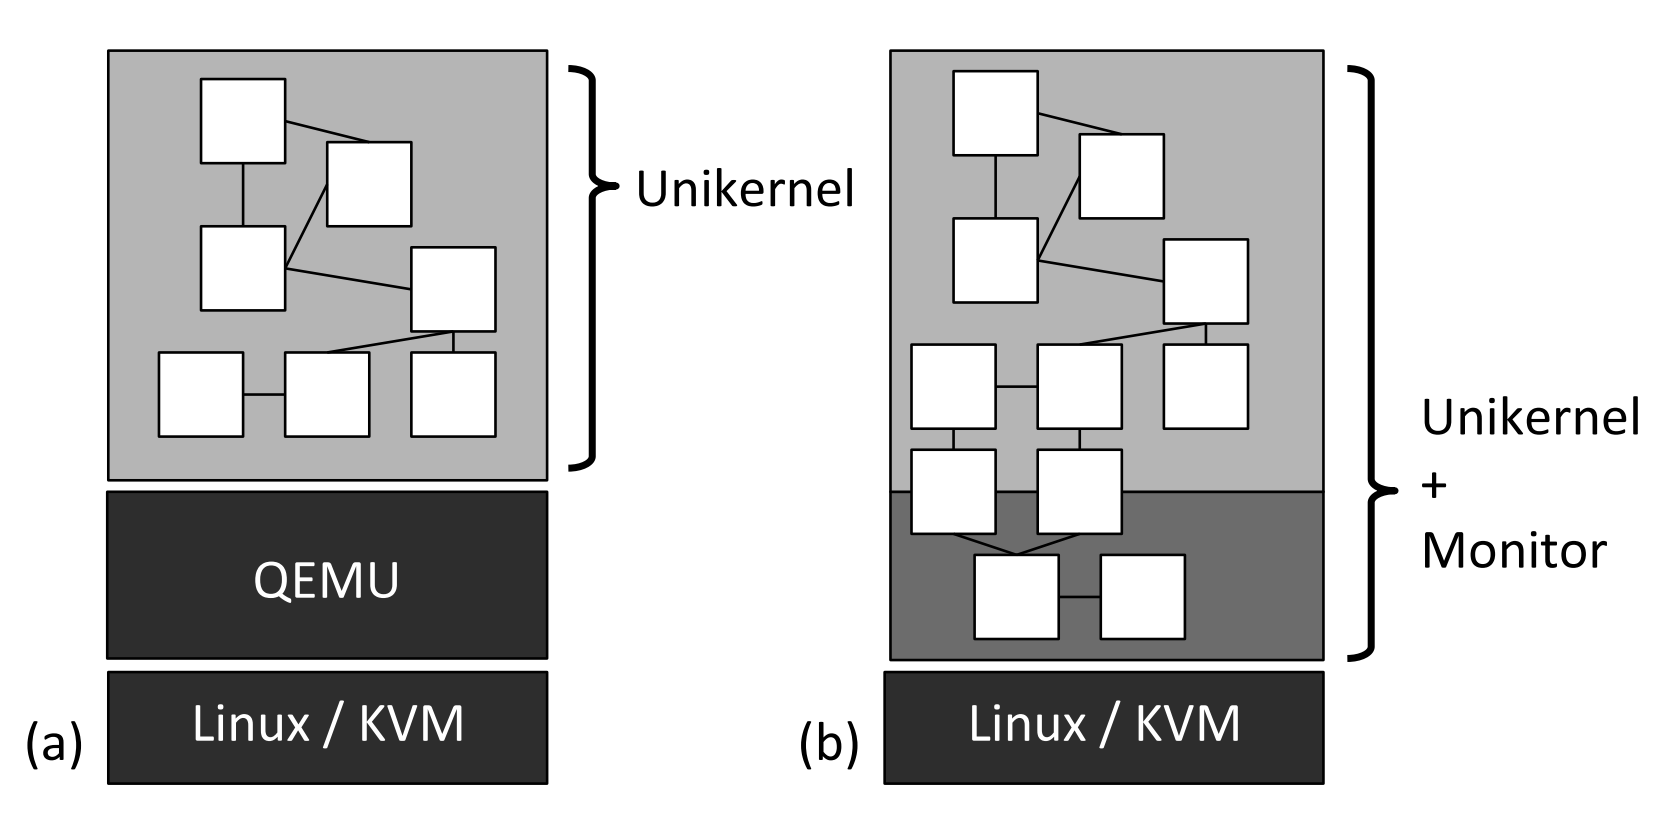
\includegraphics[width=0.8\textwidth]{figures/monitors.png}
    \caption{Unikernel Monitors: Extending Minimalism Outside of the Box \cite{Williams2016} } \label{fig:unikernel-monitor}
  \end{figure}



This thesis differs itself from the works explained above by bringing a single solution for running unikernels in Kubernetes as first class citizens and for managing unikernel-enabled IoT devices through the same interface. An easy-to-install agent can be used to run unikernels both on IoT devices and on hypervisors. It also removes the dependency to the Docker runtime completely when operating from outside the Kubernetes Master node.